% \section{Discussions}\label{sec:discuss}
% 
% This section compares \xxx and \dare's protocols (\S\ref{sec:compare}), and 
% discusses \xxx's limitations (\S\ref{sec:limits}).

\section{Comparing \xxx with \dare}\label{sec:compare}

\begin{figure}[t]
\centering
\vspace{-.4in}
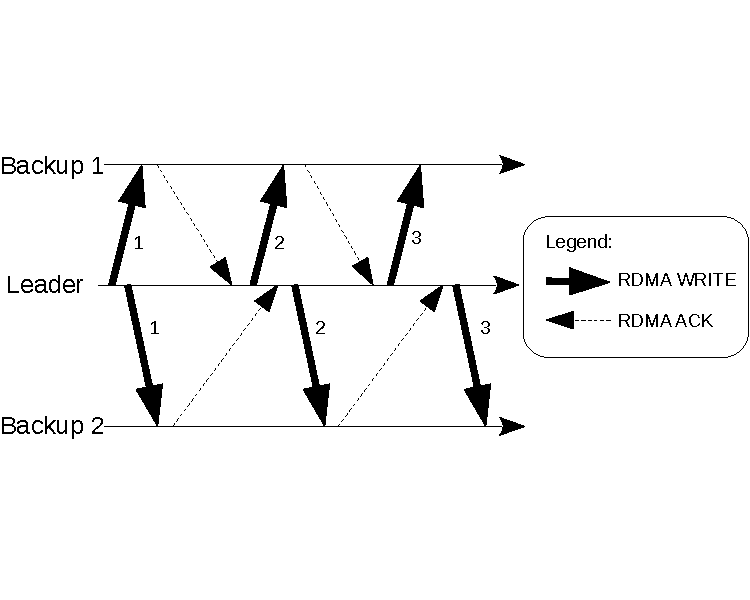
\includegraphics[width=.35\textwidth]{figures/dare_algo}
\vspace{-.53in}
\caption{{\em \dare's RDMA-based protocol.} It is a sole-leader, 
two-round protocol with three steps: (1) the leader WRITEs a consensus request 
to all backups' consensus logs and waits for ACKs to check if they succeed; 
(2) for the successful backups in (1), leader does WRITEs to update tail 
pointer of their consensus logs; and (3) on receiving a majority of ACKs in 
(2), a consensus is reached, leader does WRITEs to notify backups.}
\label{fig:dare}
\vspace{-.20in}
\end{figure}

\dare~\cite{dare:hpdc15} (Figure~\ref{fig:dare}) is one of 
the fastest \paxos protocols. It is RDMA-based and most relevant to \xxx. \dare 
is designed for both a small number of concurrent requests and 
replicas. \dare follows a sole-leader manner with two-rounds: 
first, leader does RDMA writes of consensus requests on each replica; second, 
leader does RDMA writes on each replica to update a global variable that points 
to the latest request (tail of consensus log) in each backup. \dare's both 
rounds are essential in case a backup becomes a new leader.
% Figure~\ref{fig:dare} shows 
% \dare's protocol. Figure~\ref{fig:consensus} shows \xxx's protocol.

% 
% logic uses two rounds to  wait for RDMA ACKs from backups. Our evaluation 
% shows that this protocol is fast when replica group size is small (three to 
% five), but both the ACK pollings and two-round

% It is a 
% sole-leader protocol (backups do not participate in consensus) with two rounds. 
% In the first round, the leader uses RDMA to write the consensus requests to all 
% replicas and polls RDMA ACKs to check whether the writes succeed. Second, for 
% the successful writes, the leader does another round of RDMA writes to mark the 
% writes as successful on other replicas, and poll ACKs on these writes. Once a 
% majority of successful writes in the second round, DARE reaches a consensus.

% To further improve performance, \dare makes two technical choices. First, to 
% avoid delays caused by polling ACKs, \dare uses a global RDMA CQ (Completion 
% Queue) for all replicas, making it possible to collect multiple ACKs each poll 
% operation. 

\dare is not designed to work with large concurrent requests or 
replicas for two reasons. First, its second round needs to update a global 
variable for each replica, which \emph{serializes} concurrent consensus 
requests, an essential feature for \paxos performance~\cite{paxos:practical}. 
For instance, two ongoing \dare consensus requests may interleave and cause the 
variable to point to an earlier request. Therefore, the consensus of \dare's 
new requests can not start until the consensus of prior requests finish, 
confirmed in both \dare's and our evaluation (\S\ref{sec:eval-dare}). Second, a 
sole-leader protocol is difficult to add a stable storage or 
checkpoint design. Therefore, \dare lacks durability 
(\S\ref{sec:background}), another essential \paxos 
feature~\cite{lyu1995software}.

% With these 
% two choices, \dare runs slightly faster than \xxx on three replicas.

% However, \dare is not designed to scale to a large replica group because its 
% leader does all the consensus work. Our evaluation shows that both \dare's ACK 
% pollings and its two-round consensus incurred scalability bottlenecks and had an
% approximately linear consensus latency: \dare's consensus latency increased by 
% \darescalability as replica group size increased by 35x 
% (\S\ref{sec:evaluation}).

Overall, \xxx differs from \dare in three aspects. First, \xxx's protocol has 
only one RDMA round (Figure~\ref{fig:consensus}), and \dare has two rounds. 
Second, \xxx scales well on concurrent client connections and replicas 
(\S\ref{sec:eval-dare}), and \dare~\cite{dare:hpdc15} mentioned that their 
design choices do not include scalability. Third, although \xxx is a durable 
protocol and \dare is a volatile one, \xxx is faster than \dare by \fasterDARE 
in average. \S\ref{sec:eval-dare} compares \xxx and \dare performance in 
detail.

% \subsection{\xxx Limitations}\label{sec:limits}

% Input coordination protocol.

% Have not hooked time and rand(). Can use PMP approach. Not a problem for 
% evaluated apps. 
% \xxx currently does not hook random functions such as \v{gettimeofday()} and 
% \v{rand()} because these random results are often explicit and easy to examine 
% from network outputs (\eg, a timestamp in the header of a reply). Existing 
% \paxos approaches~\cite{eve:osdi12,paxos:practical} can also be 
% leveraged to intercept these functions and make general programs produce same 
% results among replicas.
% because our output checkers have not detected network output 
% divergence comming from these functions

% Output checking protocol.

% Clamav style.
% \xxx's output checking protocol may have false positives or false negatives, 
% because it is just designed to try to improve assurance on whether replicas run 
% in sync. A server program running in \xxx may have false positive when it uses 
% multiple threads to serve the same client connection and uses these threads to 
% concurrently add outputs (\eg, \clamav in our evaluation). 
% Running a deterministic multithreading 
% scheduler~\cite{coredet:asplos10,parrot:sosp13} with the server program 
% addresses this problem.
% In our evaluation, all programs except \clamav uses only 
% one thread to process one client connection and they don't have such false 
% positives.

% A server program may also have false negative when it triggers a software bug 
% but the bug does not propagate to network outputs. From client programs' point 
% of view, such bugs do not matter. Moreover, \xxx already checkpoints file 
% system state to mitigate this issue.

% Like recent systems~\cite{dare:hpdc15,crane:sosp15}, \xxx totally orders all 
% types of requests and it has not incorporated 
% read-only optimization~\cite{eve:osdi12}, because its performance overhead 
% is already low (\S\ref{sec:overhead}). However, \xxx can be extended to 
% support read-only optimization if two conditions are met: (1) the 
% semantic an operation is read-only is clear in a server program; and (2) the 
% number of output bytes for this operation is fixed. GET requests in key-value 
% stores often meet these two conditions.

% We use GET requests to present a design. \xxx intercepts a client program's 
% outbound socket calls (\eg, \send), compares the first three bytes in each call 
% with ``GET". If they match, \xxx appends two extra \xxx metadata fields 
% \v{read\_only} and \v{length} in this outbound call to the server. \xxx then 
% intercepts a server's \recv calls and strips these two fields. If the first 
% field is true, \xxx directly processes this operation in a local replica 
% and strips the next \v{length} bytes from the output checker within the same
% connection. In sum, \xxx processes these operations locally without making 
% outputs across replicas diverge.

% When execution divergence is detected in a replica, \xxx's rollback mechanism 
% is not designed to guarantee that the re-executions of this replica will 
% definitely avoids this divergence. We made this design choice because both 
% our evaluation and a previous work Eve~\cite{eve:osdi12} found that divergence 
% happens extremely rarely in evaluation. In our evaluation, we found that simply 
% re-executing the log can practically make \xxx's replicas converge to 
% same execution states. A similar finding is that although Eve provided a 
% sequential re-execution approach to with divergence avoidance guarantee, which 
% \xxx can leverage, but even Eve's evaluation didn't experience any divergence 
% and thus this approach was not invoked.

% Read only opt?

% No guarantees on recovery. Best effort. But, can we actually server requests 
% one by one?

%% No lxc.

%% Support for Java may not be good due to the VM memory copying. Some 
% techniques that avoid memory copying may be usable~\cite{weixu:tsinghua}. Good 
% for % C/C++ programs as long as they use POSIX socket APIs.




% Another promising direction is three-phase commit (3PC): 3PC is often 
% blamed by its intolerance on network partitions and asynchronour 
% communications, 
% and its high latency caused by the three round-trips. Fortunately, within the 
% RDMA-enabled datacenter context, people may leverage \xxx's techniques and 
% experience to build a significantly faster and more reliable 3PC protocols.

% Other replication topics.

% Parallel program analysis. Such a short coordination time can make replicas 
% run almost as fast as each other, support many time-critical analyses 
% such as race detection and security defenses.


% TBD: use \xxx to detect software bugs by checking outputs, even in 
% real-world deployments. XXX make program % inputs strongly consistent across 
% replicas, so output divergence are likely % from software bugs. XXX promising 
% 
% results in our evaluation. Find a bug in % ssdb?

% One idea: can leverage the checkpoint and rollback protocok, and the 
% consensus part, to build a system that can automatically bypass concurrency 
% bugs without fixing them. The way to bypass: proactively reordering socket 
% calls. Self-healing system.

% A core building block in future operating systems. Maintain a consistent view 
% of computing resources and data. Used in scheduling framework (Mesos) because 
% its latency is almost compatible with context switches of processes (sub 
% milli seconds).





% \subsection{\xxx Has Broad Applications}\label{sec:apps}
% 
% In addition to greatly improving \paxos scalability of many systems in 
% datacenters, we envision that \xxx can be applied in broad areas, and here we 
% elaborate three. First, \xxx's RDMA-accelerated \paxos protocol and its 
% implementation could be a template for other replication protocols (\eg, 
% byzantine fault-tolerance~\cite{zyzzyva:sosp07,pbft:osdi99}). 





% Second, by efficiently constructing multiple, equivalent executions for the 
% same program, \xxx can benefit distributed program analysis techniques. 
% Bounded 
% by the limited computing resources on single machine, recent advanced 
% program analysis frameworks become 
% distributed~\cite{decouple:usenix08, speck:asplos08, 
% shadowreplica:ccs13, wester:parallelizing:asplos13,repframe:apsys15} in order 
% to 
% offload analyses on multiple machines. \xxx can be leveraged in these 
% frameworks so that developers of analysis tools can just focus on their own 
% analysis logic, while \xxx's general replication architecture handles the 
% rest.
% 
% Moreover, program analyses developers can tightly integrate their tools with 
% \xxx. For instance, they can proactively diversify the orders of socket calls 
% in \xxx's consensus logs among replicas to improve replicas' tolerance on 
% security attacks~\cite{con:hotpar12}.



% Third, \xxx can be a core building block in the emerging datacenter operating 
% systems~\cite{matei:hotcloud11, mesos:nsdi11, datacenter:os}. As a 
% datacenter continuously emerges a computer, an OS may be increasingly needed for 
% such a giant computer. \xxx's fast, scalable coordination service is especially 
% suitable for such an OS's scheduler to maintain a consistent, reliable view on 
% both computing resources and data in a datacenter. For instance, \xxx's 
% latency is about 30 \us even with over 100 replicas, smaller than a 
% process context switch (tens to hundreds of \us).
